The earthquake has produced some already expected situations such as chaotic
traffic, despair among the population, etc., which has also generated some kind
of uncertainty at the data. For example, the keyword ``\emph{bridge}'' has been
mentioned multiple times, which suggests a structural problem that could've
ended in collapse if analysing the isolated word. However, by analysing the
whole context by means of a bar chart of retweets frequency, as shown in
Figure~\ref{fig:re_bridge_vbar}, we can see that most mentions refer to closing
bridges instead of reporting physical problems at the bridge.

\begin{figure}[!h]
    \centering
    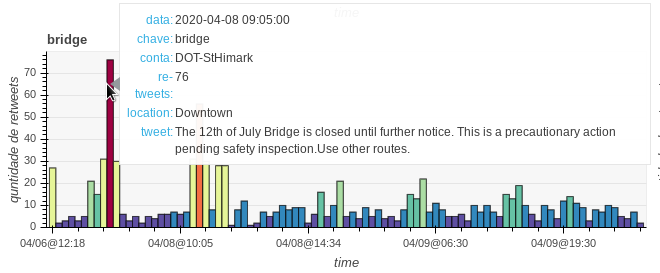
\includegraphics[width=0.95\textwidth]{figs/q3/re_bridge_vbar.png}
    \caption{Bridge closed}
    \label{fig:re_bridge_vbar}
\end{figure}

Another point is with respect to fake news. At 8:00~AM of Apr 8th a tweet
appeared to alarm users about an eventual tsunami, and a lot of retweets have
followed to spread the ``news''. However, as reported on Apr 9th at 9:00~AM, the
city's unique geography prevents such disaster to happen, and according to the
greater number of retweets of this second information we can infer this is the
real truth about tsunamis in St. Himark.

\begin{figure}[!h]
    \centering
    \begin{subfigure}[!h]{0.47\textwidth}
        \centering
        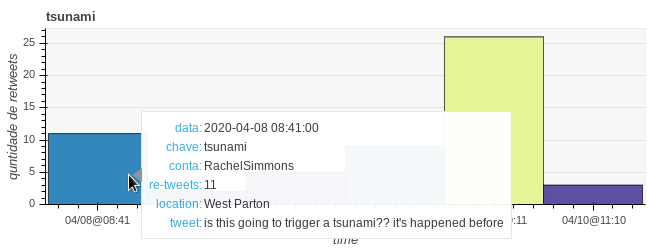
\includegraphics[width=1.00\textwidth]{figs/q3/re_tsunami_fake.png}
        \caption{Tsunami fake}
        \label{fig:re_tsunami_fake}
    \end{subfigure}
    \begin{subfigure}[!h]{0.47\textwidth}
        \centering
        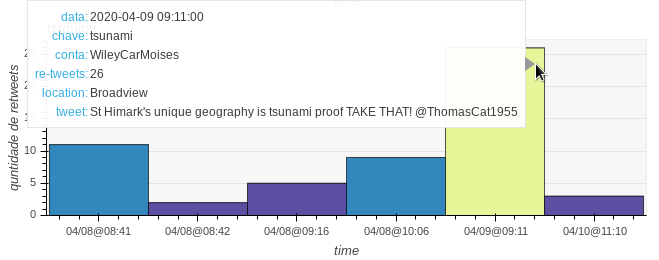
\includegraphics[width=1.00\textwidth]{figs/q3/re_tsunami_truth.png}
        \caption{Tsunami truth}
        \label{fig:re_tsunami_truth}
    \end{subfigure}
    \caption{Tsunami fake news}
    \label{fig:re_tsunami}
\end{figure}

A third discovery made through the retweets frequency bar chart is that there
was a circus show going on in town at the same week, and that after the disaster
that endend with buildings collapsing, the elephants started to be used to help
lifting heavy blocks of rocks in an attempt to search for people or corpses.

\begin{figure}[!h]
    \centering
    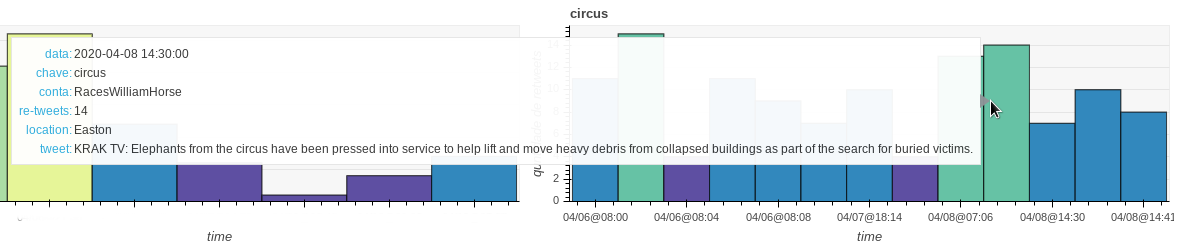
\includegraphics[width=0.95\textwidth]{figs/q3/re_circus.png}
    \caption{Circus elephants}
    \label{fig:re_circus}
\end{figure}

